\chapter{Classical Multidimensional Scaling with Perturbation}
\label{sec:dmcs}
\chaptermark{CMDS with Perturbation}

\section{Review of Classical Multidimensional Scaling}
\label{sec:cmds} 
Given an $n \times n$ hollow symmetric dissimilarity
matrix $D$, and an embedding dimension $d$, we seek $X \in
\mathbb{R}^{n \times d}$, where the rows $X_1, X_2, \dots, X_n \in
\mathbb{R}^d$ of $X$ represent coordinates of points in $\R^d$, such
that the overall inter-point distances between $X_i$ and $X_j$ are
as close as possible to the distances given by the dissimilarity
matrix $D$. For a given matrix $H$, we shall denote by $H^{(2)} = H
\circ H$ the element-wise squaring of the matrix $H$.
Given $D$, classical multidimensional scaling 
involves the following steps:
\begin{enumerate}
  \item Compute the matrix $B = -\frac{1}{2}P D^{(2)} P$ where $P = I - 1_n1_n^{\top}/n$ is the double centering matrix. Here $I$
denotes the $n \times n$ identity matrix and $1_n = (1, \dots,
1)^\top \in \mathbb{R}^n$.
  \item Extract the $d$ largest positive eigenvalues $s_1, \dots, s_d$
of $B$ and the corresponding eigenvectors ${u}_1, \dots, u_d$.
  \item Let $X = U_B S_B^{1/2} \in \mathbb{R}^{n \times d}$, where
$U_B = (u_1, \dots, u_d)$ and $S_B = \textrm{diag}(s_1, \dots,
s_{d})$. Each row of $X$ represents the coordinate of a point in
$\R^d$.
\end{enumerate} 
In essence, the procedure minimizes the Strain loss
function defined as $L(X) = \| XX^{\top} - B \|_{F}$ where
$\|\cdot\|_{F}$ denote the Frobenius norm of a matrix. Furthermore,
the resulting configuration ${X}$ centers all points around the origin, resulting in an inherent issue of identifiability: $X$ is
unique only up to an orthogonal transformation. In the following
presentation, we will write $X = U_B S_B^{1/2} W$ where $W$ is some
orthogonal matrix, for a suitably transformed $X$.

\section{Noise Models and Embedding}
\subsection{Model 1: $\Delta^2 = D^2 + E$}
\label{sec:M&E} In this section we propose three different but
related noise models for the matrix of observed dissimilarities.
Suppose that we have a latent or unobserved matrix $D$ of inter-point Euclidean distances between $n$ points in $\mathbb{R}^d$,
i.e. $D_{ij} = \|x_i - x_j\|$. Let $D^{(2)}$ denote the entry-wise
square of $D$ and $\Delta$ be the observed dissimilarity matrix, such
as that measured via a scientific experiment.

The first noise model we consider is $\Delta^{(2)} = D^{(2)} + E$ 
% \label{D^2+E} An error model proposed in \cite{DsquaredplusE} for
% $\Delta$ is $\Delta^2 = D^2 + E$, 
where we think of $D^{(2)}$ as the signal matrix and $E$ as the noise
matrix; see also \citet{DsquaredplusE}. We shall assume that $E$
satisfies the following conditions:
\begin{enumerate}[]
  \item[(i)] $\mathbb{E}[E] = 0$, hence $\mathbb{E}[\Delta^{(2)}] = D^{(2)}$.
  \item[(ii)] The matrix $E$ is hollow and symmetric.
  \item[(iii)] The entries $E_{ij}$ are independent and $\mathrm{Var}(E_{ij}) = \sigma^2$.
  \item[(iv)] There exists a finite constant $C$ such that $E_{ij}$
    follows a sub-Gaussian distribution with variance proxy $C$ 
    for all $i,j$, i.e., $\mathbb{P}[E_{ij} \geq t] \leq
    2\exp(-t^2/(2C))$ for all $i,j$. 
\end{enumerate}

\subsection{Model 2: $\Delta = D + E$}
\label{D+E} 
The second error model we consider is $\Delta = D + E$. We once more require that the random matrix $E$ satisfies conditions (i) to
(iv) identical to that in the model $\Delta^{(2)} = D^{(2)} + E$ along
with a constant third and fourth
moment conditions, i.e., there exists finite constants $\gamma$
and $\xi$ such that (v) $\mathbb{E} [E_{ij}^3] \equiv \gamma$ and $\mathbb{E}
[E_{ij} ^ 4] \equiv \xi$ for all $i,j$.
%\end{equation}

\subsection{Model 3: Matrix Completion}
\label{matrix_completion} 
Finally, we consider a noise model where only a fraction of the
entries of $D$ are observed. More specifically, for a given $q \in [0,1]$ let
$\Delta$ be such that for $i < j$, with probability $q$ we observe $\Delta_{ij} = D_{ij}$ and with probability $1 - q$, $\Delta_{ij}$ is
unobserved in which case we set $\Delta_{ij} = 0$. We then have
$\Delta = D + E$ where $E_{ij}$ is distributed as $(- D_{ij}) \times \mathrm{Bernoulli}(1-q)$. Furthermore, $\mathbb{E}[\Delta] = q \cdot
D$ and $E[\Delta^{(2)}] = q \cdot D^{(2)}$. This model is motivated
by the widely-studied problems of distance matrix completion and sensor
localization; see e.g.,
\citet{Javanmard2013,Chatterjee,Alfakih1999, wirelesssensor}. 

For each of the above noise models, we shall apply classical
multidimensional scaling to the observed $\Delta$ to obtain a
configuration matrix $\hat{X}$ whose rows are the estimate of the latent,
unobserved $X =  [x_1, \dots, x_n]^{\top}$. A natural question that arises is how the added
noise affects the embedding configuration. That is, what is the
relationship between the configuration $X$ and $\hat{X}$ obtained from classical
multidimensional scaling of $D$ and $\Delta$ ?


\section{Related Works}
\label{RW} The problem of recovering an Euclidean distance matrix from
noisy or imperfect observations of pairwise dissimilarity scores
arises naturally in many different contexts. For example, in
\cite{DsquaredplusE}, the authors considered the model $\Delta^{(2)} = D^{(2)} +
E$ along with the estimator
$$\hat{D}^{(2)} = \argmax_{M \in \mathcal{D}^{(2)}_n} \Bigl\{ \frac{1}{2} \|\Delta^{(2)} - M\|_{F}^2 + \lambda_n \mathrm{trace} \,\,(-\frac{1}{2}PMP) \Bigr \}$$ 
for $D^{(2)}$. Here $\mathcal{D}^{(2)}_n$ is the set of $n \times n$
{\em squared} Euclidean distance matrix and $\lambda_n$ is a tuning
parameter. Corollary 6 in \cite{DsquaredplusE} states that under suitable model on $E$, with probability approaching to one we have 
\begin{equation}
\label{eq:zhang}
\|\hat{D}^2 - D^2 \|_F^2 \leq 36n\sigma^2(r+1)
\end{equation}
where $\sigma$ is the variance of the noise and $r$ is the rank of
$D^{2}$.  In this paper we obtain, as a corollary of ours results, a
bound of the same order on $\|\hat{D}^2 - D^2\|_{F}^2$. Furthermore,
our central limit theorem on the configuration matrix $\hat{X}$
provides a more refined limiting result, albeit one of a different
flavor from Eq.~\eqref{eq:zhang}.

On the other hand, completing a distance matrix with missing entries
has been a popular problem in the engineering and social sciences;
see, for example, \cite{Alfakih1999,Bakonyi,Singer9507, Spence1974}
. Distance matrix completion is closely related to multidimensional
scaling \citep{BGbook,Chatterjee, Javanmard2013, Montanari}. Especially
noteworthy is Theorem~2.5 of \cite{Chatterjee}, where the author
established an upper bound for the mean squared error on the estimator
$\tilde{M}$ for a general distance matrix $M$. More specifically, let
$(K,d)$ be a compact metric space and $x_1, \dots, x_n$ be $n$
arbitrary points in $K$. Let $M$ be the $n \times n$ matrix whose
$ij$-entry is $d(x_i,x_j)$. Let $\epsilon > 0$ be such that $q \geq
n^{-1 + \epsilon}$. For a given $\delta > 0$, let $N(\delta)$ be the
covering number of $K$ using balls of radius $\epsilon$ with respect
to the metric $d$. Then there exists an estimator $\tilde{M}$ obtained
by truncating the singular value decomposition of $M$ such that
$$ \mathrm{MSE}(\tilde{M}) \leq C \inf_{\delta > 0} \min \Bigl\{  \frac{\delta + \sqrt{ N(\delta/4) /n}}{\sqrt{q}} , 1 \Bigr \} + C(\epsilon) e^{-ncq}$$
where $c$ and $C$ are constants depending on the truncation level $\eta$ for 
the singular values of $M$ and $C(\epsilon)$ is a constant depending only on $\epsilon$ and $\eta$. Of particular interest is the application of this theorem to the
Euclidean distance matrix, for which we obtain roughly
$$\textrm{MSE} (\tilde{M}) \leq \frac{Cn^{-1/3}}{\sqrt{q}}.$$ 
Another recent result for the configuration $\hat{X}$ obtained from the incomplete distance matrix $\Delta$
is Theorem~1 of \cite{Taghizadeh} which states that, with high
probability
$$\|\hat{X} - X\|_F \leq \mathcal{O}\Bigl(\frac{\sqrt{n}}{\sqrt{q}}\Bigr).$$ 
Our central limit theorem in this paper improves upon both results.  It is worth mentioning that the Euclidean distance matrix completion problem can also be
viewed from an optimization point of view. See
\cite{Tasissa2018ExactRO} for a review of such approaches.


%%%%%%%%%%%%%%%%%%%%%%%%%%%%%%%%%%%%%%%%%%%%%%%
\section{Main Theorems}
\label{main}

Recall that a random variable $X$ is sub-Gaussian if $\mathbb{P}[ | X
| > t] \leq 2 e^{ -\frac{t^2}{ {K}^2} }$ for some constant $K$ and for
all $t \geq 0$.  Associated with a sub-Gaussian random variable is a
Orlicz norm defined as $ \| X \|_{\psi_2} = \inf \{ t >0 : \mathbb{E}
\exp(\frac{X^2 }{t^2}) \leq 2 \}$.  A random vector $X$ in $\R^n$ is
called sub-Gaussian if the one-dimensional marginals $\big \langle X,
x \big \rangle$ are sub-Gaussian random variables for all $x \in
\R^n$, and the corresponding sub-Gaussian norm of $X$ is defined as
$\|X\|_{\psi_2} = \sup\limits_{x \in S^{n-1}} \| \big \langle X, x
\big \rangle \|_{\psi_2}$.


We now present central limit theorems for
the rows of the classical multidimensional scaling configuration $\hat{X}$ for the three noise
models in \S~\ref{sec:M&E}. Intuitively speaking, the theorems
established that the rows of $\hat{X}$, after some orthogonal
transformation, is approximately normally distributed around the rows
of $X$. Furthermore, the covariance matrix will depend on the noise
model and the true distribution of the points in the underlying space
and are substantially different between the three noise models
considered. In particular, the covariance matrix for the noise model
$\Delta^2 = D^2 + E$ in Theorem~\ref{main_theorem_D^2+E} depends only
on the variance $\sigma^2$ of the noise $E_{ij}$.  This is in contrast
with the covariance matrices of the model $\Delta = D + E$ and the
model $\mathbb{E}[\Delta] = q D$ in Theorem~\ref{main_theorem_D+E} and
Theorem~\ref{main_theorem_matrix_completion}, both of which depend
also on the underlying true distances $D_{ij}$. The machinery involved
in proving these results are by and large the same and we refer the
reader to the Appendix for a sketch of the proof. For ease of
exposition, we denote by $(A)_i$ the $i$-th row of a matrix.  

\begin{theorem}[central limit theorem for $\Delta^2 = D^2 + E$]
\label{main_theorem_D^2+E}%
Let $Z_1, \dots, Z_n$ be independent and identically distributed
according to a multivariate sub-Gaussian distribution $F$ on $\R^d$. Let $D$ be the Euclidean
distance matrix generated by the $Z_k$'s, i.e. $D_{ij} = \|Z_i -
Z_j\|$. 
Let $\Delta^2 = D^2 + E$ where the noise matrix $E$ satisfy the conditions (i) $\mathbb{E}[E] = \bm{0}$, (ii) $E$ is hollow and
symmetric, (iii) the entries $E_{ij}$ are independent for $i \leq j$
with $\mathrm{Var}[E_{ij}] \equiv \sigma^2$, and (iv) each $E_{ij}$
follows a sub-Gaussian distribution.  Denote by $\hat{X}_n$ the
classical multidimensional scaling embedding configurations of
$\Delta$ into $\mathbb{R}^{d}$. There exists a sequence of $d
\times d$ orthogonal matrices $\{W_n\}_{n=1}^{\infty}$ such that for
any $\alpha \in \mathbb{R}^{d}$ and any fixed row index $i$, we have
$$ \lim_{n {\to} \infty} \mathbb{P} \{n^{1/2} [(\hat{X}_n W_n)_i - (Z_i - \bar{Z}) ]\leq \alpha\} = \Phi(\alpha, \Sigma) $$
  where $\bar{Z}$ is the mean of $Z_k$'s and $\Phi(\alpha, \Sigma)$
denotes the cumulative distribution function of a multivariate Gaussian with mean $0$ and
covariance matrix $\Sigma$, evaluated at $\alpha$.  Here $\Sigma =
\frac{\sigma^2}{4} {\Xi}^{-1}$ where $\Xi = \mathrm{cov}(Z_k) \in
\R^{d \times d}$.
\end{theorem}

\begin{remark} We can relax the common variance requirement (iii) in
Theorem~\ref{main_theorem_D^2+E}. Let $\textrm{Var}(E_{ij}) =
\sigma_{ij}^2$ and suppose that, for a fixed $i$, the collection $(D^{2}_{ij} -
\Delta^{2}_{ij})(Z_{j} - \mathbb{E}[Z_j])$ for $j \not = i$ satisfies the conditions for the
Lindeberg-Feller central limit theorem. Let $\Sigma_{i} = n^{-1}
\sum_{j} \sigma_{ij}^2 \mathrm{cov}(Z_k)$. We 
obtain the following variant of Theorem \ref{main_theorem_D^2+E}:
$$n^{1/2} \Sigma_{i}^{-\frac{1}{2}} \bigl((\hat{X_n}W_n)_i - (Z_i - \bar{Z})\bigr) \rightarrow \mathcal{N}(0, I).$$
\end{remark}

\begin{theorem}[Central Limit Theorem for $\Delta = D + E$]
\label{main_theorem_D+E}%
Let $Z_1, \dots, Z_n$ be independent and identically distributed
according to a multivariate sub-Gaussian distribution $F$ on $\R^d$. Let $D$ be the Euclidean
distance matrix generated by the $Z_k$'s, i.e. $D_{ij} = \|Z_i -
Z_j\|$. 
Let $\Delta = D + E$ and suppose that the noise matrix $E$ satisfy, in addition to the
conditions in Theorem~\ref{main_theorem_D^2+E}, the condition (v)
$\mathbb{E}[E_{ij}^3] \equiv \gamma$ and $\mathbb{E}[E_{ij}^4] \equiv
\xi$. Denote by $\hat{X}_n$ the classical multidimensional embedding of
$\Delta$ into $\R^d$. There exists a sequence of $d \times d$
orthogonal matrices $\{W_n\}_{n=1}^{\infty}$ such that for any $\alpha
\in \mathbb{R}^{d}$ and any fixed row index $i$,
  $$ \lim_{n {\to} \infty} \mathbb{P} \{n^{1/2} \bigl((\hat{X}_n W_n)_{i} - (Z_i - \bar{Z})\bigr) \leq \alpha\} = \int 
  \Phi(\alpha, \Sigma(z)) dF(z)$$
  where $\bar{Z}$ is the mean of $Z_k$'s and $\Phi(\alpha, \Sigma)$
  denotes the cumulative distribution function of a multivariate
  Gaussian with mean $0$ and covariance matrix $\Sigma$, 
evaluated at $\alpha$. Here $\Sigma (z)= {\Xi}^{-1}
\widetilde{\Sigma}(z) {\Xi}^{-1}$ where $\Xi =
\mathrm{cov}(Z_i) \in \R^{d \times d}$ and, 
with $\mu = \mathbb{E}[Z_i] \in \mathbb{R}^{d}$,
  $$\widetilde{\Sigma} (z) = \mathbb{E}_{Z_k}\Bigl[(\sigma^2
  \|z - Z_k\|^2 + \gamma \| z - Z_k \|+ \frac{1}{4} \xi -
  \frac{\sigma^4}{4}) (Z_k- {\mu}) (Z_k - {\mu})^\top\Bigr] $$  
is a covariance matrix depending on $\emph{z}$.
\end{theorem}

%\begin{remark}
%Intuitively, this theorem claims that the rows of $\hat{X}$, after some orthogonal transformation, is approximately normal around the rows of $X$. Furthermore, the covariance matrix will depend on the noise and the true distribution of the points in the underlying space.
%\end{remark}

\begin{theorem}[Central Limit Theorem for $\Delta = D$ with missing entries]
\label{main_theorem_matrix_completion} Let $Z_1, \dots, Z_n$ be
independent and identically distributed according to a multivariate sub-Gaussian distribution $F$ on $\R^d$. Let $D$ be the
Euclidean distance matrix generated by the $Z_i$'s, i.e. $D_{ij} =
\|Z_i - Z_j\|$. Suppose that with probability $q_n \in [0,1]$ we
observe the distance $D_{ij}$ and with probability $1 - q_n$ it is
missing, i.e., $\Delta = D + E$ where $E_{ij} = (- D_{ij}) \times
\mathrm{Bernoulli}(1-q_n)$. Denote by $\hat{X}_n$ the classical
multidimensional embedding of $\Delta$ into $\R^d$.  Then there exists a sequence
of $d \times d$ orthogonal matrices $\{W_n\}_{n=1}^{\infty}$ such that
if $n q_n = \omega(\log^{4}{n})$, then for any $\alpha \in
\mathbb{R}^{d}$ and any fixed row index $i$,
  $$ \lim_{n {\to} \infty} \mathbb{P} \{n^{1/2} [(\hat{X_n}W_n)_{i} - q_n^{1/2} (Z_i - \bar{Z})] \leq \alpha\} = \int \Phi(\alpha, \Sigma(z)) dF(\emph{z})$$
  where $\bar{Z}$ is the mean of $Z_i$'s and $\Phi(\alpha, \Sigma)$ denotes the CDF of a multivariate Gaussian with mean $0$ and covariance matrix $\Sigma$, evaluated at $\alpha$. Here $\Sigma (z)= {\Xi}^{-1} \widetilde{\Sigma}(z) {\Xi}^{-1}$, $\Xi = \mathrm{cov}(Z_i) \in \R^{d \times d}$ and with $\mu = \mathbb{E}[Z_i] \in \mathbb{R}^{d}$,
  $$\widetilde{\Sigma} (z) = \frac{1-q_n}{4} \times \mathbb{E}_{Z_k} \Bigl[ \|z - Z_k\|^4 (Z_k- {\mu}) (Z_k - {\mu})^\top\Bigr]$$ 
  is a covariance matrix depending on $z$. 
\end{theorem}
\begin{remark}
We emphasize that, in the statement of Theorem~\ref{main_theorem_matrix_completion}, 
$(\hat{X_n}W_n)_{i}$ is centered around $q_n^{1/2}(Z_i - \bar{Z})$ and not around $Z_i - \bar{Z}$. Therefore, unless $q_n$ is known or that an identifiability condition is specified, the classical multidimensional scaling configuration $\hat{X}_n$ will only recovers an estimate of $Z - 1_n \bar{Z}$ up to an orthogonal transformation $W_n$ and a scaling factor $q_n^{1/2}$.
\end{remark}

%%%%%%%%%%%%%%%%%%%%%%%%%%%%%%%%%%%%%%%%%%%%%%%%%
\section{Empirical Results}
\label{ER}

\subsection{Three Point-mass Simulated Data}
\label{SD}

As a simple illustration of our central limit theorem, we embed noisy Euclidean
distances obtained from $n$ points into $\R^2$. For illustrative purpose, we will focus on the error model $\Delta = D
+ E$ as in Theorem
\ref{main_theorem_D+E}. Experimental results for the other error
models are completely analogous. We consider three
points $x_1,x_2,x_3 \in \mathbb{R}^2$ for which the inter-point
distances are 3,4 and 5 (these three points form a right triangle) and
generate $n_k = \pi_k n$ points equal to $x_k$, $k=1,2,3$, where $\pi
= [0.2,0.3,0.5]^\top$.  The resulting Euclidean inter-point distance
matrix $D$ is then subjected to uniform noise, yielding $\Delta = D+E$
where $E_{ij} \iid \textrm{Uniform}(-4,+4)$ for $i<j$ and
$E_{ij}=E_{ji}$.  For this setting, our central limit theorem for the classical multidimensional embedding of $\Delta$ into $\mathbb{R}^{2}$ yields class-conditional Gaussians.  For $n \in \{50,
100, 1000\}$, Figure \ref{fig:Simulation result} compares, for
one realization, the theoretical vs.\ estimated means and covariances
matrices (95\% level curves).  Table \ref{tab:cov_1} shows the
empirical covariance matrix for one of the point masses,
$\hat{\Sigma}^{(1)}$, behaving in accordance with Theorem
\ref{main_theorem_D+E}. %:-)

Table \ref{tab:cov_1} investigates the empirical covariance matrix for
one of the point masses, and its entry-wise variance, as a function of
$n$. The theoretical covariance matrix is $$\Sigma^{(1)}
= \begin{bmatrix} 13.56 & -3.06 \\ -3.06 & 22.65 \end{bmatrix}$$

%%%%%%%%%%%%%%%%%%%%%%%%%%%%%%%% this is the table with two columns %%%%%%%%%%%%%%%%%%%%%%%%%%%%%%%%
{
\centering
\begin{table}
\begin{tabular}{ c c c c c c  }
\toprule
\textbf{}  & $n$=50 & $n$=100 & $n$=500 & $n$=1000\\
\midrule\\
\addlinespace[-2ex]
$\hat{\Sigma}^{(1)}:$ &
$  \begin{bmatrix}  14.15 & 0.25 \\ 0.25 &  79.07 \end{bmatrix}$ &
$  \begin{bmatrix} 13.67 & -0.79 \\ -0.79 & 98.96 \end{bmatrix}$ &
$ \begin{bmatrix}  13.65 & -2.34 \\ -2.34 &  41.02 \end{bmatrix}$ &
$ \begin{bmatrix} 13.63 & -2.70 \\ -2.70 & 31.76 \end{bmatrix}$ &\\
\addlinespace[2ex]
$\mathrm{Var}\begin{bmatrix}
           \hat{\Sigma}^{(1)}_{11} \\
           \hat{\Sigma}^{(1)}_{12} \\
           \hat{\Sigma}^{(1)}_{22} \end{bmatrix}:$ &
$  \begin{bmatrix}  41.25 \\ 113.31 \\  829.52 \end{bmatrix}$&
$  \begin{bmatrix} 19.29  \\ 68.06 \\ 984.45 \end{bmatrix}$ &
$ \begin{bmatrix}  3.67 \ \\ 7.87 \\  31.71 \end{bmatrix}$ &
$ \begin{bmatrix} 1.71  \\ 3.25 \\ 11.08 \end{bmatrix}$ &\\
\addlinespace[1ex]
\bottomrule
\end{tabular}
\caption{Empirical average of covariance matrix $\hat{\Sigma}^{(1)}$, and entry-wise variance (500 simulations).}
\label{tab:cov_1}
\end{table}
}

\begin{remark}
In this simulation we relax the requirement that the entries of $\Delta$ should be nonnegative in order to illustrate the phenomenon of decreasing covariance with increasing $n$. 
\end{remark}

\begin{figure}[htbp]
    \centering
    \subfloat[$n$=50]{{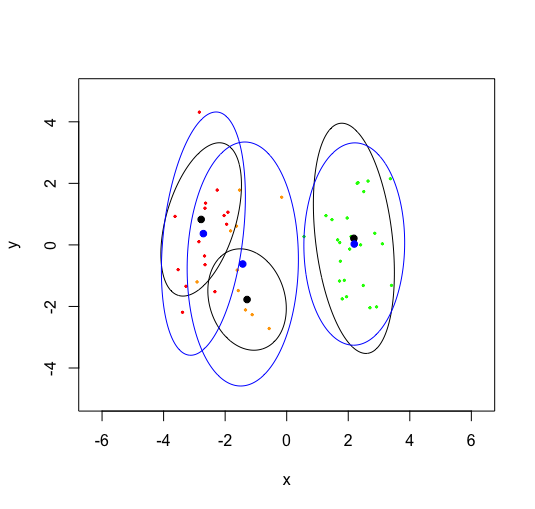
\includegraphics[width=.4\textwidth]{./figure/n_50_D+E_2.png} }}
    \quad
    \subfloat[$n$=100]{{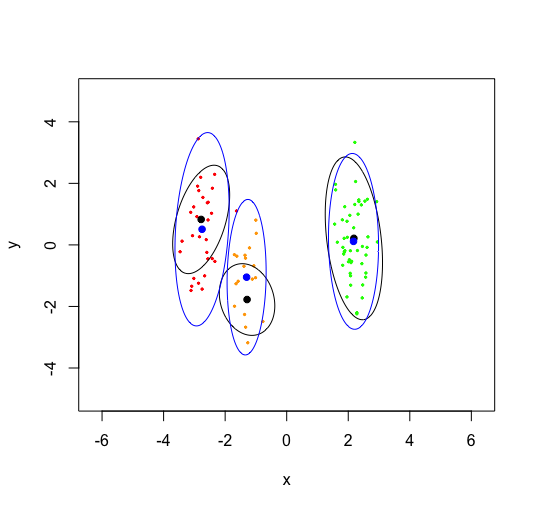
\includegraphics[width=.4\textwidth]{./figure/n_100_D+E_2.png} }}
    \quad
    \subfloat[$n$=500]{{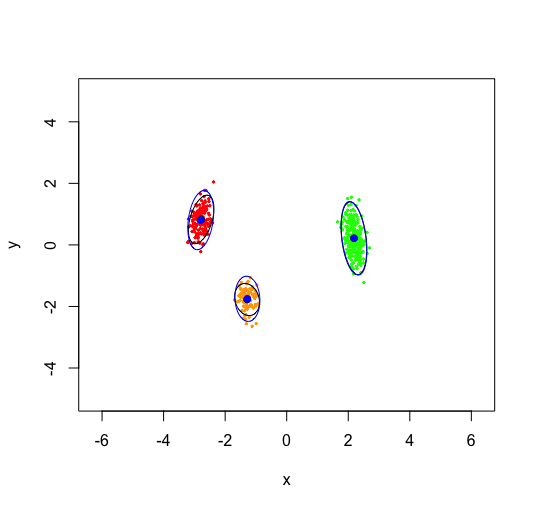
\includegraphics[width=.4\textwidth]{./figure/n_500_D+E_2.png} }}
    \quad
    \subfloat[$n$=1000]{{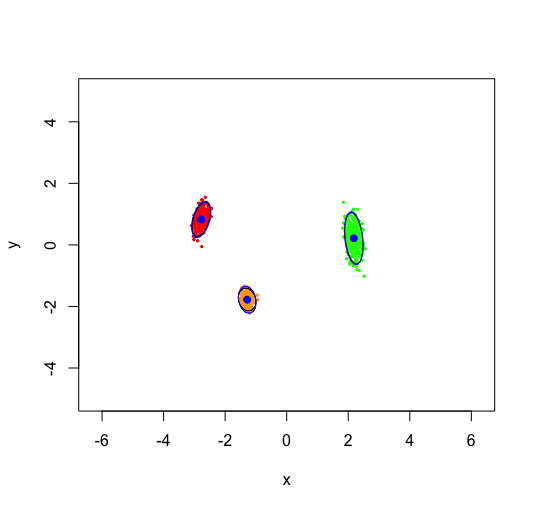
\includegraphics[width=.4\textwidth]{./figure/n_1000_D+E_2.png} }}
    \caption{Simulation results for $n$=50, 100, 500 and 1000 points, as described in Section \ref{SD}. The blue ellipses are the 95\% level curves of the empirical covariance matrix, and the blue dots are the empirical centers for three classes. The black dots are the true positions of $x_1$, $x_2$ and $x_3$, and the black ellipses are the 95\% level curve for the theoretical covariance matrices as in Theorem \ref{main_theorem_D+E}. Note that the blue and black centers and ellipses coincide for large $n$.}%
    \label{fig:Simulation result}%
\end{figure}

\subsection{Shape clustering}
As a second illustration of the effect of noise on CMDS, we examine a more involved clustering experiment in the (non-Euclidean) shape space of closed curves. In this experiment, we consider boundary curves obtained from silhouettes of the Kimia shape database. Specifically, we restrict attention to three predefined classes of objects (bottle, bone, and wrench) and take from each class three different examples of shapes all given by planar closed polygonal curves representing the objects' outline. Figure \ref{fig:bottle_bone_wrench} shows one instance for each of the bottle, bone, and wrench class. A database of noisy curves is then created as follows: for each of the nine template shapes, we generate 100 noisy realizations in which vertices of the curve are moved along the curve's normal vectors with random distances drawn from independent Gaussian distributions at each vertex. This results in a total of 900 noisy versions of the initial curves such as the ones displayed in Figure \ref{fig:noisy_bottle_bone_wrench}.

\begin{figure}[htp]
    \centering
    \subfloat[Bottle]{{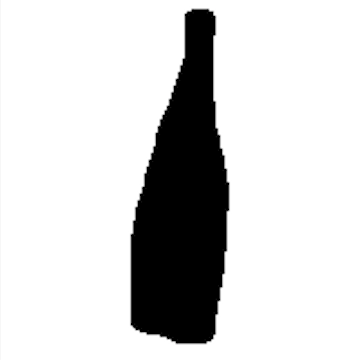
\includegraphics[width=.25\textwidth]{./figure/bottle_0} }}
    \quad
    \subfloat[Bone]{{
\includegraphics[width=.25\textwidth]{./figure/bone_0} }}
    \quad
    \subfloat[Wrench]{{
\includegraphics[width=.25\textwidth]{./figure/wrench_0} }}
    \caption{Examples from the Kimia Dataset.}
    \label{fig:bottle_bone_wrench}
\end{figure}

\begin{figure}[htp]
    \centering
    \subfloat[Bottle]{{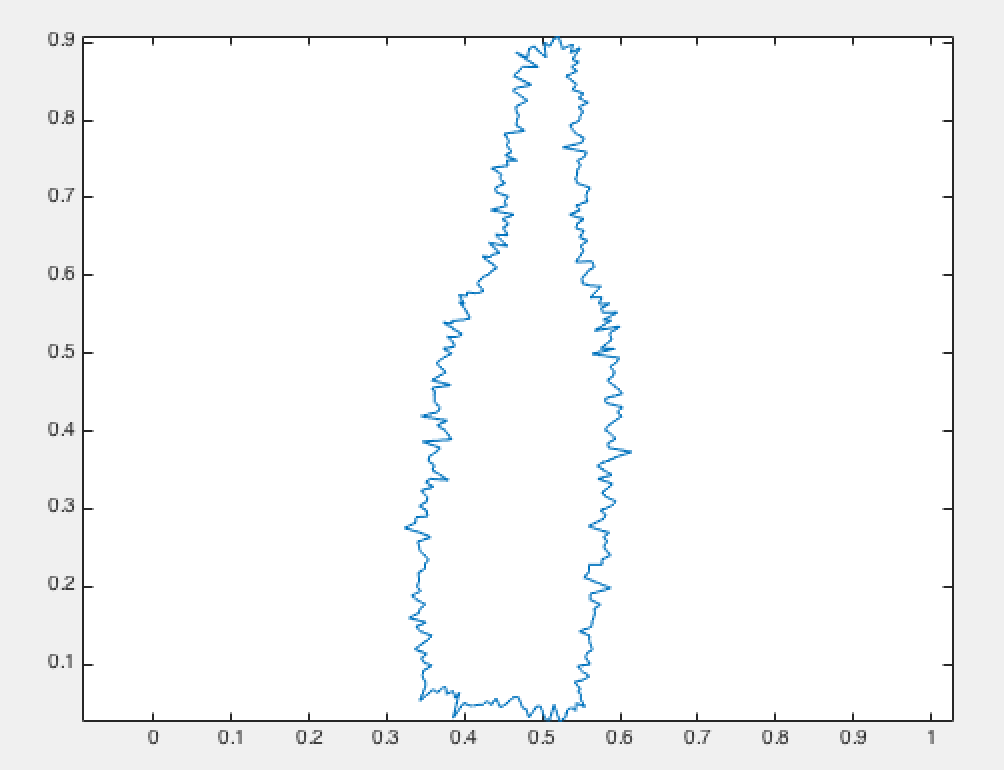
\includegraphics[width=.25\textwidth]{./figure/bottle} }}
    \quad
    \subfloat[Bone]{{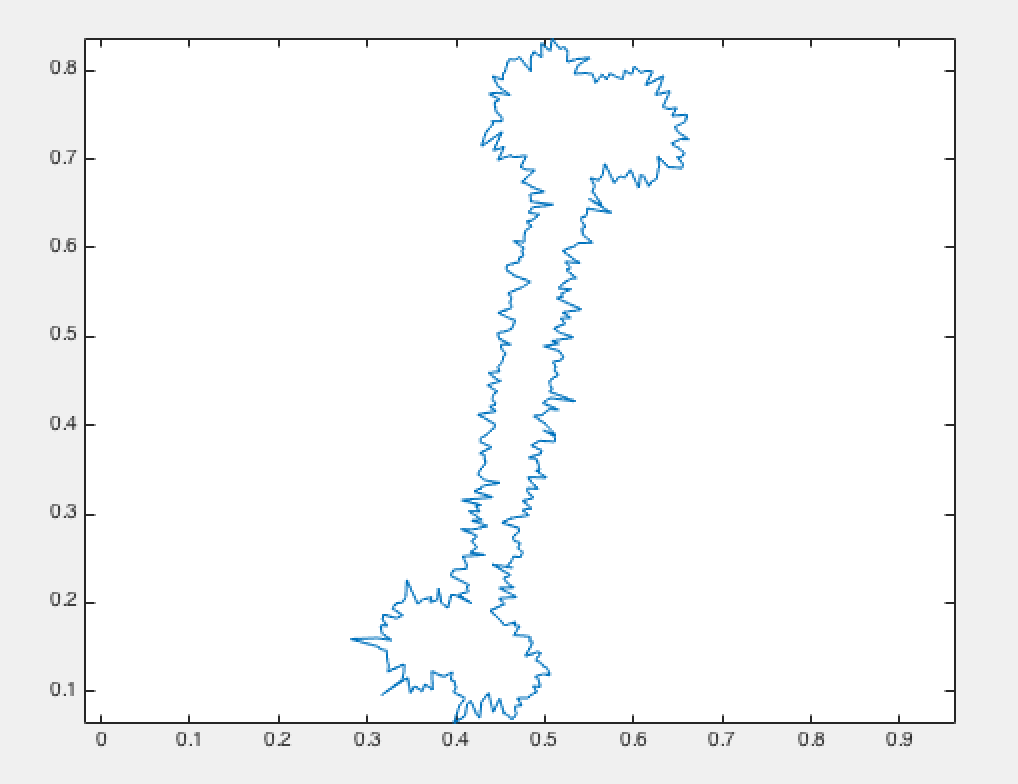
\includegraphics[width=.25\textwidth]{./figure/bone} }}
    \quad
    \subfloat[Wrench]{{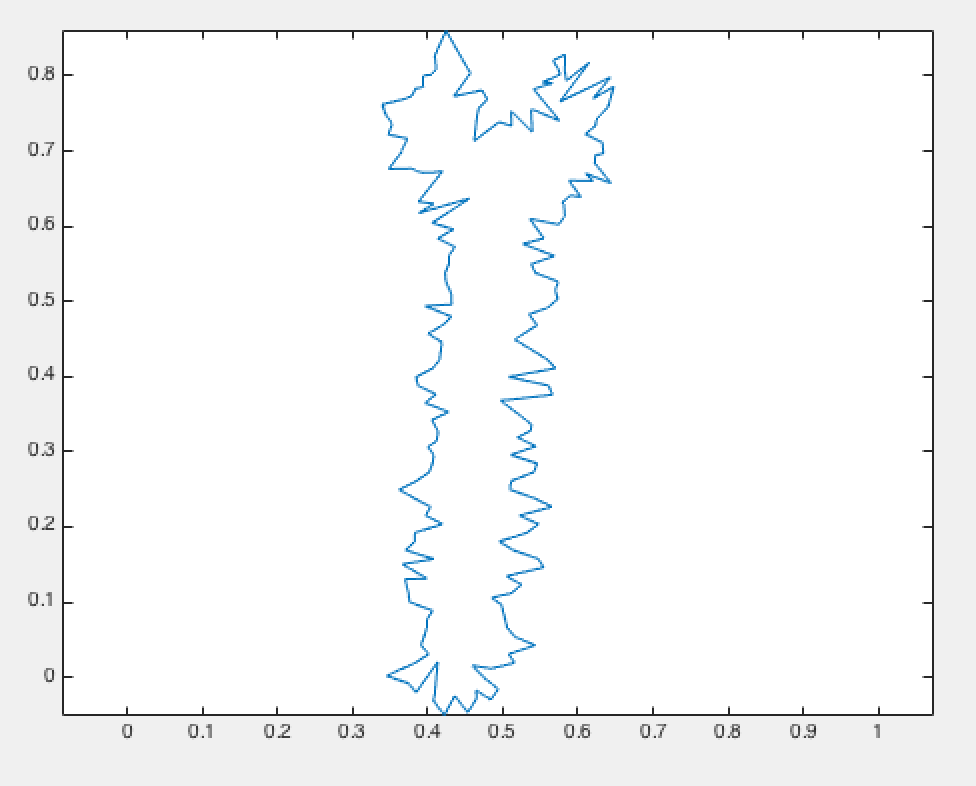
\includegraphics[width=.25\textwidth]{./figure/wrench} }}
    \caption{Noisy versions of examples from the Kimia Dataset.}
    \label{fig:noisy_bottle_bone_wrench}
\end{figure}

We then compute the pairwise distance matrix between all the curves (including the noiseless templates) based on a shape distance which was introduced in \cite{Glaunes2008} and later extended in the work of \cite{Kaltenmark2017}. This type of metric is based on the representation of shapes in a particular distribution space called currents, see \cite{Kaltenmark2017} for details. In our context, this metric offers several advantages: (i) the distance is completely geometrical in the sense that it is independent of the sampling of the curves and does not rely on predefined pointwise correspondences between vertices; (ii) it has an intrinsic smoothing effect that provides robustness to noise to a certain degree; (iii) it can be computed in closed form with minimal computational time which is critical given the large number of pairwise distances to evaluate. In this setting, we can view the resulting distance matrix as a perturbation of the ideal distances between the 9 template curves, which fits into the generic framework of our model. (Note that we leave aside the issue of checking the technical assumptions on the matrix $E$, which may be quite involved for this noise model and distance.)

We proceed to perform CMDS on this distance matrix. A scree plot investigation
%A dimension reduction procedure
shows that an appropriate embedding dimension here is $\hat{d} = 3$ (the top three eigenvalues are 2.20, 0.68, 0.06 with the fourth $\ll$ 0.01).
%\cite{Zhu&Ghodsi}. 
The resulting embedding configuration is shown in Figure \ref{fig:large currents}. 
This configuration exhibits nine fairly well-separated clusters roughly centered around the position of each of the noiseless template curves. Those, in turn, form 3 `super-clusters' consistent with the classes. Furthermore, the ellipsoidal shape of each cluster suggests that the configuration approximately follows a Gaussian distribution.

\begin{figure}[htp]
\centering
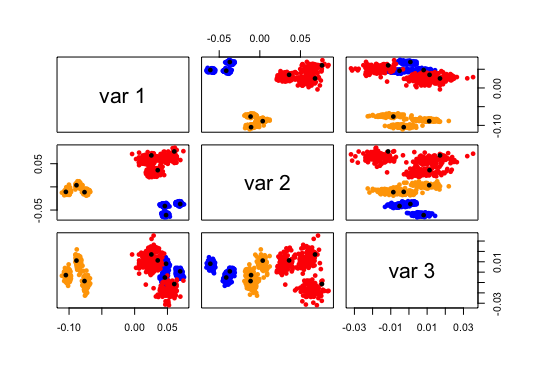
\includegraphics[scale=0.9]{./figure/Pairs_plot_noisy_total_linear_909.png}
\caption{Pairs plot of CMDS into $\mathbb{R}^3$ for the noisy curves. Colors correspond to the different classes (blue for bottle, red for bone, and orange for wrench). The position of the nine template curves in the configuration are highlighted with large black dots.}
    \label{fig:large currents}
\end{figure}

While these preliminary shape clustering results are obtained with a specific and simple distance on the space of curves, future work will investigate whether similar properties hold with different, more elaborate metrics and/or geometric noise models. The central limit theorem derived here could then constitute a useful theoretical tool to evaluate the discriminating power of shape clustering methods based on CMDS.

%%%%%%%%%%%%%%%%%%%%%%%%%%%%%%%%%%%%%%%%%%%%%%%%%%%%%%%%%%%
\section{Discussion}
\label{D}

In \citet{Athreya2016} and \citet{OMNI}, the authors prove that adjacency spectral embedding of the random dot product graph gives rise to a central limit theorem for the estimated latent positions. In this work we extend these results to the previously unexplored area of perturbation analysis for CMDS, addressing a gap in the literature as acknowledged in \citet{Fan} and \citet{Peterfreund&Gavish}. Notably, the three noise models we proposed in Section \ref{sec:M&E} each give rise to a central limit theorem; that is, for Euclidean distance matrix, the rows of the configuration matrix given by CMDS under noise will center around the corresponding rows of the true configuration matrix. Furthermore, our simulations on the synthetic data together with the shape clustering data all demonstrated the validity of our results. We have avoided any discussion of the model selection problem of choosing a suitable embedding dimension $\hat{d}$. Instead, we assume $d$ is known -- except in Section 4.2. There are many methods for choosing (spectral) embedding dimensions, see \cite{Zhu&Ghodsi, Jackson, Chatterjee}. 

\begin{figure}[tp]
    \centering
    \subfloat[$n$=50]{{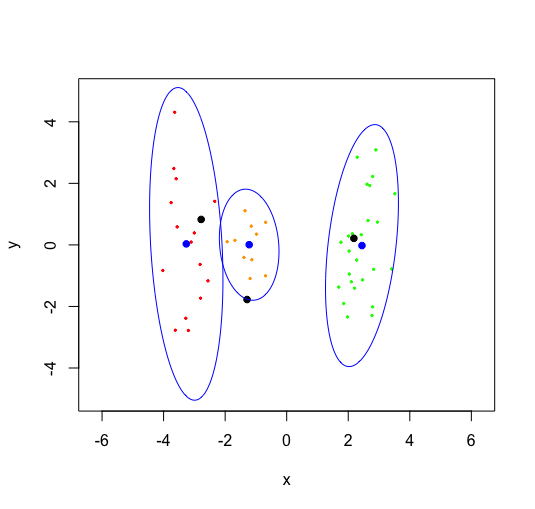
\includegraphics[width=.4\textwidth]{./figure/Uncommon_var_E_n_50.png} }}
    \quad
    \subfloat[$n$=100]{{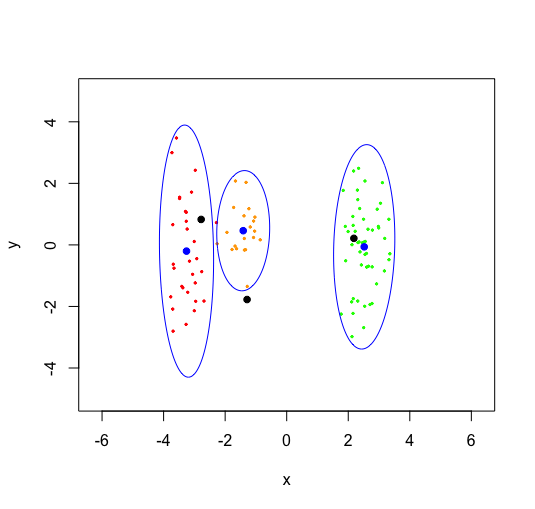
\includegraphics[width=.4\textwidth]{./figure/Uncommon_var_E_n_100.png} }}
    \quad
    \subfloat[$n$=500]{{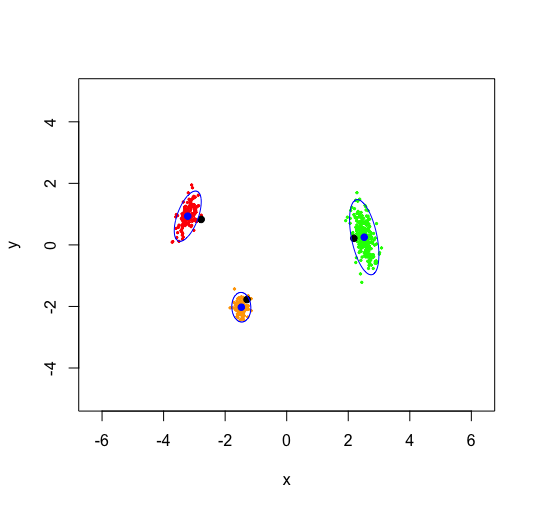
\includegraphics[width=.4\textwidth]{./figure/Uncommon_var_E_n_500.png} }}
    \quad
    \subfloat[$n$=1000]{{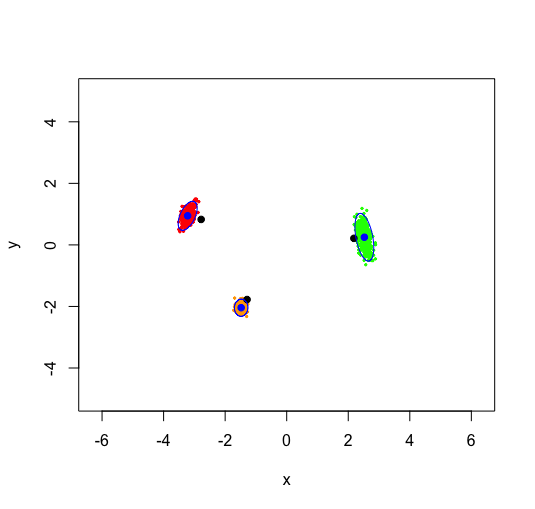
\includegraphics[width=.4\textwidth]{./figure/Uncommon_var_E_n_1000.png} }}
    \caption{Simulation of CMDS with heteroscedastic noise $\widetilde{E}$. The black dots are the true positions for the three points. The blue dots are the empirical means and the blue ellipses are the 95\% level curve of the empirical covariance matrix. Note that $\widetilde{E}$ used in this simulation is of the same order for the off-diagonal blocks as that used in Figure \ref{fig:Simulation result}. NB: there is asymptotic bias.}
    \label{fig:Uncommon_var_E}
\end{figure}

A practically relevant and conceptually illustrative example comes from relaxing the assumption of common variance for the entries of the noise matrix $E$ in Section \ref{D+E}: the consistency result from Theorem \ref{main_theorem_D+E} no longer holds. To illustrate this point, we return to our three-point-mass simulation presented in Section \ref{SD} and modify our noise model as follows: Let $\widetilde{E}_{ij} \iid \textrm{Uniform}(-D_{ij}, +D_{ij})$ for $i < j$ and $\widetilde{E}_{ij}= \widetilde{E}_{ji}$. (The noise now depends on the entries of $D$, and $\Delta = D + \widetilde{E}$ no longer has negative entries.) The embedding of $\Delta$ into two dimensions gives class-conditional Gaussians; however, we have introduced bias into the embedding configuration. Figure \ref{fig:Uncommon_var_E} shows, for one realization, the embedding result. Note that the empirical mean and the theoretical positions do not coincide in simulation with large $n$, and theoretically even in the limit.
\begin{figure}[tp]
    \centering
    \subfloat[$n$=50]{{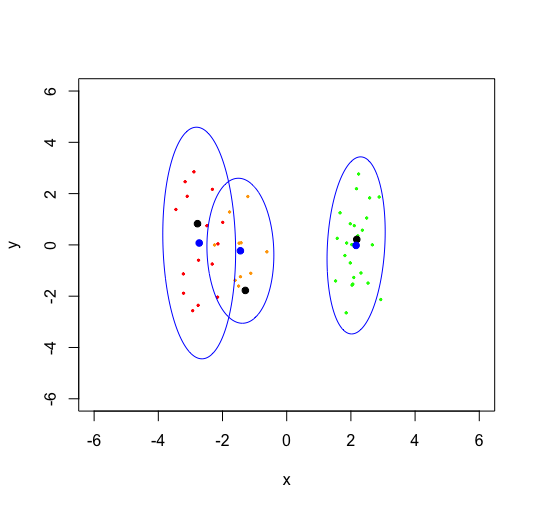
\includegraphics[width=.4\textwidth]{./figure/raw_stress_n_50.png} }}
    \quad
    \subfloat[$n$=100]{{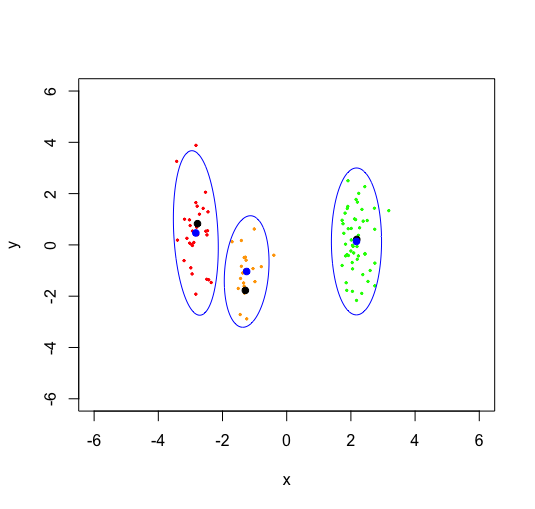
\includegraphics[width=.4\textwidth]{./figure/raw_stress_n_100.png} }}
    \quad
    \subfloat[$n$=500]{{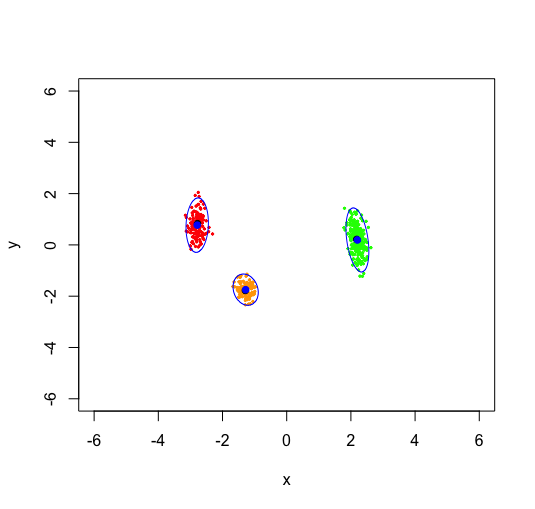
\includegraphics[width=.4\textwidth]{./figure/raw_stress_n_500.png} }}
    \quad
    \subfloat[$n$=1000]{{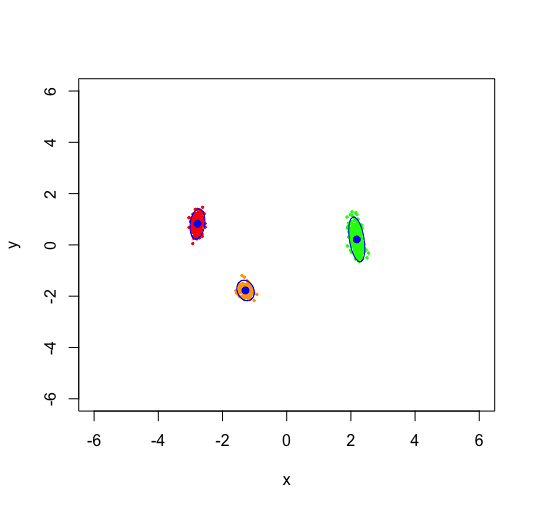
\includegraphics[width=.4\textwidth]{./figure/raw_stress_n_1000.png} }}
    \caption{Simulation of MDS using raw stress criterion for $n$=50, 100, 500 and 1000 points.
                  The black dots are the true positions of $x_1$, $x_2$ and $x_3$, the blue dots are the empirical mean of the simulation and the blue ellipses are the 95\% level curve of the empirical covariance matrix.}
    \label{fig:RawStress}
\end{figure}

CMDS is just one of a wide variety of multidimensional scaling techniques. Minimizing the raw stress criterion is another commonly used MDS technique \citep{Leeuw-Heiser}, i.e., given a $n \times n$ observed dissimilarity matrix $\Delta$ and an embedding dimension $d$, one seeks to minimize the objective function $$\sigma_r = \sigma_r(X) = \sum\limits_{(i,j)} (\delta_{ij} - \|X_i - X_j\|)^2.$$ The minimization of $\sigma_r(X)$ is with respect to all configurations $X \in \mathbb{R}^{n \times d}$ and usually proceeds via an iterative algorithm which updates the configuration matrix $X$ until a stopping criterion is met. Keeping the simulation settings as in Section \ref{SD},  the resulting configuration is shown in Figure \ref{fig:RawStress}. This suggests that the CLT may hold for raw stress just as well as for CMDS. However, this claim is at best a conjecture at present as perturbation analysis of stress minimization algorithms is significantly more involved.
%%%%%%%%%%%%%%%%%%%%%%%%%%%%%%%%%%%%%%%%%%%%%%%%%%%%%%%%%%%
\section{Application: Omni Embedding of graphs and Hypothesis Testing}










%%%%%%%%%%%%%%%%%%%%%%%%%%%%%%%%%%%%%%%%%%%%%%%%%%%%%%%%%%%%%%
\section{Proof of the Theorems}

\subsection{Proof of Theorem \ref{main_theorem_D+E}}
\label{proof}
We proceed to give a complete proof for Theorem \ref{main_theorem_D+E}. Theorems \ref{main_theorem_D^2+E} and \ref{main_theorem_matrix_completion} will have different covariance matrix structures then what is given in Lemma \ref{appthm3} and will be dealt with later.

Given a matrix $A$, we denote by $\| A \|$ and $\|A\|_{F}$ its spectral and Frobenius norm, respectively.
We will utilize the following observation repeatedly in our presentation.
\begin{observation}
\label{appthm1}
 Let $A$ and $B$ be matrices of appropriate dimensions. Then 
 $$\|A B\|_F = \|B^{\top} A^{\top}\|_{F} \leq \min\{ \|A\| \times \|B\|_F, \|B\| \times \|A\|_{F}\}.$$
\end{observation}

We remind our readers the following notations for the subsequent presentation. 
 Recall that $B = -\tfrac{1}{2} P D^{(2)} P$ and $\hat{B} = -\frac{1}{2} P \Delta^{(2)} P$ are the double centering of $D^{(2)}$ and $\Delta^{(2)}$, respectively. If $D^{(2)}$ 
is a Euclidean distance matrix whose elements are $D_{ij} = \|Z_i -Z_j\|$, then $B = P Z Z^{\top} P$. In particular, $U_B S_B^{1/2} = P Z \tilde{W}$ for some $d \times d$ orthogonal matrix $\tilde{W}$. The $i$th row of $U_B S_B^{1/2}$ is then $\tilde{W}_n^{\top} (Z_i - \bar{Z})$. Now let $W^{*}$ be the orthogonal matrix satisfying $W^{*} = \argmin_{W} \|U_B^{\top} U_{\hat{B}} - W\|_{F}$. %Our main goal is to investigate the quantity $\hat{X} - U_B S_B^{1/2} W^* $. 
The following lemma provides a decomposition for $\hat{X} - U_B S_B^{1/2} W^*$ into a sum of several matrices. 
%%%%%%%%%%%%%%%%%%%%%%%%%%%%%%%%%%%%%%%%%%%%%%%%%%%%%%%%%%%%%%%%%%%%%
\begin{lemma}
\label{appthm2}
  Let $W^{*}$ be the orthogonal matrix satisfying $W^{*} = \argmin_{W} \|U_B^{\top} U_{\hat{B}} - W\|$. Then 
      \begin{align}
          \hat{X} - U_B S_B^{1/2} W^*  &=   ( \hat{B} - B) U_B S_B^{-1/2} W^{*}  \label{term1}\\
          & - (\hat{B} - B) U_B (S_{B}^{-1/2} W^{*} - W^{*} S_{\hat{B}}^{-1/2})  - U_B U_B^{\top} (\hat{B} - B) U_B W^* S_{\hat{B}}^{-1/2}      \label{term3}\\
          & + (I - U_B U_B^{\top}) (\hat{B} - B) (U_{\hat{B}} - U_B W^{*}) S_{\hat{B}}^{-1/2}     \label{term4}\\
          & + U_B (U_B^{\top} U_{\hat{B}} - W^*) S_{\hat{B}}^{1/2} + U_B (W^{*} S_{\hat{B}}^{1/2} - S_B^{1/2} W^{*})     \label{term6}
    \end{align}
\end{lemma}
\begin{proof}
We have 
        \begin{align*}
          \hat{X} - U_B S_B^{1/2} W^*  
          & = U_{\hat{B}} S_{\hat{B}}^{1/2} - U_B W^* S_{\hat{B}}^{1/2} + U_B (W^* S_{\hat{B}}^{1/2} - S_{B}^{1/2} W^*) \\
          & = U_{\hat{B}} S_{\hat{B}}^{1/2} - U_B U_B^{\top} U_{\hat{B}} S_{\hat{B}}^{1/2} + U_B U_B^{\top} U_{\hat{B}} S_{\hat{B}}^{1/2} - U_B W^* S_{\hat{B}}^{1/2} + U_B (W^* S_{\hat{B}}^{1/2} - S_{B}^{1/2} W^*) \\
          & = (I - U_B U_B^{\top}) \hat{B} U_{\hat{B}} S_{\hat{B}}^{-1/2} + U_B (U_B^{\top} U_{\hat{B}} - W^{*}) S_{\hat{B}}^{1/2} + U_B (W^* S_{\hat{B}}^{1/2} - S_{B}^{1/2} W^*) \\
          &= (I - U_B U_B^{\top}) (\hat{B} - B) U_{\hat{B}} S_{\hat{B}}^{-1/2} + U_B (U_B^{\top} U_{\hat{B}} - W^*) S_{\hat{B}}^{1/2} + U_B (W^* S_{\hat{B}}^{1/2} - S_{B}^{1/2} W^*). 
        \end{align*}
        We used the facts $ U_B U_B^\top B = B$ and $U_{\hat{B}} S_{\hat{B}}^{1/2} = \hat{B} U_{\hat{B}} S_{\hat{B}}^{-1/2}$ in the above equalities. The last two terms of the above display is Eq.~\eqref{term6}. Denote by $R$ the term  
        $(I - U_B U_B^{\top}) (\hat{B} - B) U_{\hat{B}} S_{\hat{B}}^{-1/2}$, we have
        \begin{equation*}
        \begin{split}
        R & 
            =  (I - U_B U_B^{\top}) (\hat{B} - B) ( U_BW^* + U_{\hat{B}} - U_{B} W^{*}) S_{\hat{B}}^{-1/2}   \\
          & = (\hat{B} -B) U_B W^* S_{\hat{B}}^{-1/2} - U_B U_B^{\top} (\hat{B} - B) U_B W^* S_{\hat{B}}^{-1/2} + (I - U_B U_B^{\top}) (\hat{B} - B) (U_{\hat{B}} - U_{B} W^{*}) S_{\hat{B}}^{-1/2} 
          \\
          & = ( \hat{B} - B) U_B S_B^{-1/2} W^{*} 
           - (\hat{B} - B) U_B (S_{B}^{-1/2} W^{*} - W^{*} S_{\hat{B}}^{-1/2}) 
           - U_B U_B^{\top} (\hat{B} - B) U_B W^* S_{\hat{B}}^{-1/2} \\
           & + (I - U_B U_B^{\top}) (\hat{B} - B) (U_{\hat{B}} - U_{B} W^{*})S_{\hat{B}}^{-1/2}
           \end{split}
        \end{equation*}
        The four terms in the above display are identical to that in Eq.~\eqref{term1} through Eq.~\eqref{term4}.
\end{proof}

 Lemma~\ref{appthm2} implies
 $$\hat{X} {W^*}^{\top} \tilde{W}_n - U_B S_B^{1/2} \tilde{W}_n = \hat{X} {W^*}^{\top} \tilde{W}_n - PZ = (\hat{B} - B) U_B S_B^{-1/2} \tilde{W}_n + R_n \tilde{W}_n$$ where $R_n$ are the matrices in Eq.~\eqref{term3} through Eq.~\eqref{term6}. The essential term is $(\hat{B} - B) U_B S_B^{-1/2} \tilde{W}_n$. We analyzed the rows of this matrix in Lemma~\ref{appthm3} where we show that they converge to multivariate normals. Meanwhile, Lemma~\ref{appthm4} shows that the rows of the matrices $R_n$, when scaled by $n^{1/2}$, converge to $0$ in probability. Combining these results yield Theorem 2. A few minor changes to the covariance computation in the proof of Lemma~\ref{appthm3} also yield Theorem~\ref{main_theorem_D^2+E} and Theorem~\ref{main_theorem_matrix_completion}.
  % the matrix $W_n$ in the statment of Theorem 2 is then $W_n{W^*}^{\top} \tilde{W}_n$ Indeed, the term $\hat{X} {W^*}^{\top} \tilde{W}_n$ can be denoted by $\hat{X} W_n$ for some orthogonal matrix ${W}_n= {W^*}^{\top} \tilde{W}_n$ identical to that in the statement of Theorem 1,2, and 3, while the rows of $U_B S_B^{1/2} \tilde{W}_n$ is, as we observed earlier, simply $(Z_i - \bar{Z})$. 

\begin{lemma}
\label{appthm3}
  Let $Z_1, \dots, Z_n$ be independent and identically distributed according to some multivariate sub-Gaussian distribution F. Then there exists a sequence of $d \times d$ orthogonal matrices $\tilde{W}_n$, such that for any fixed index $i$ with $Z_i = z_i$, we have
  $$ n^{1/2} \tilde{W}_n^{\top} [(\hat{B} - B) U_B S_B^{-1/2}]_{i} \longrightarrow \mathcal{N}(0, \Sigma(z_i))$$
  where $\Sigma (z_i) = {\Xi}^{-1} \widetilde{\Sigma}(z_i) {\Xi}^{-1}$, 
  $\Xi = \mathbb{E}[Z_k{Z_k}^\top] \in \mathbb{R}^{d \times d}$, ${\mu} = \mathbb{E}[Z_k] \in \R^d$ and 
  $$\widetilde{\Sigma} (z_i) = \mathbb{E}_{Z_k}[(\sigma^2 \|z_i - Z_k\|^2 + \mathbb{E}[E_{ij}^3] \|z_i - Z_k \|+ \frac{1}{4} \mathbb{E}[E_{ij}^4] - \frac{\sigma^4}{4}) (Z_k- {\mu}) (Z_k - {\mu})^\top] \in \mathbb{R}^{d \times d}$$  is a covariance matrix depending on $z$. Here $(A)_i$ or $[A]_i$ denote the $i$th row of a matrix $A$. 
\end{lemma}
\begin{proof}
 Recall that $PZ = U_B S_B^{1/2} \tilde{W}_n $. We therefore have
    \begin{align*}
        n^{1/2} \tilde{W}_n^\top [(\hat{B} - B) U_B S_B^{-1/2}]_{i}
        & = n^{1/2} \tilde{W}_n^\top [(\hat{B} - B) PZ \tilde{W}_n^\top {S_B}^{-1}]_{i} \\
        & = n^{1/2} \tilde{W}_n^\top {S_B}^{-1} \tilde{W}_n [(\hat{B} - B)PZ]_{i}\\
        & = - n^{1/2} \tilde{W}_n^\top {S_B}^{-1} \tilde{W}_n [P(D \circ E  + \frac{E^2}{2} )PZ]_{i}\\
        & = - n^{1/2} \tilde{W}_n^\top {S_B}^{-1} \tilde{W}_n \Bigl[ P \Bigl(D \circ E + \frac{E^2 - \sigma^2 1_n 1_n^{\top}}{2}\Bigr) P Z\Bigr]_{i}
    \end{align*}
The last equality holds since  $P 1_n = 0$. Now $PZ = Z - 1_n \bar{Z} = Z - 1_n \mu^{\top} + \tilde{R}_n$ where $\|\tilde{R}_n\| = O(n^{-1/2})$ with high probability.  
Therefore,
    \begin{equation*}
   % \label{eq:6}
    \begin{split}
        n^{1/2} \tilde{W}_n^\top [(\hat{B} - B) U_B S_B^{-1/2}]_{i} 
         =& - n \tilde{W}_n^\top S_B^{-1} \tilde{W}_n \Bigl[n^{-1/2} \sum_{j \neq i}^{n} \Bigl(D_{ij} E_{ij} + \frac{E_{ij}^2 - \sigma^2 1_n 1_n^{\top}}{2} \Bigr) (Z_j - \mu)\Bigr] \\ &+ o(1) %\\ 
       % & - \frac{1}{\sqrt{n}} (D \circ E + \frac{E^2 - \sigma^2 \boldsymbol{1}\boldsymbol{1}^\top}{2})_{ii} (X- \boldsymbol{1} \mu^{\top})_{i} ].
    \end{split}
    \end{equation*} 
Conditioning on $Z_i = z_i$ and ignoring the term $o(1)$ that vanishes as $n \rightarrow \infty$, the above expression is sum of $n-1$ independent mean $0$ random vector. We then invoke the Lindeberg-Feller central limit theorem to show that this sum converges to a multivariate normal. We now evaluate the covariance matrix for this sum. Each summand has covariance matrix of the form
\begin{align*}
\mathrm{cov}[(E_{ij} D_{ij} + \frac{E_{ij}^2 - \sigma^2}{2}) (Z_j - {\mu})]
& = \mathrm{Var}\Bigl(E_{ij} \|z_i - Z_j\| + \frac{E_{ij}^2 - \sigma^2}{2}\Bigr) (Z_j - {\mu}) (Z_j - {\mu})^\top.
\end{align*}
%We now consider $\mathrm{Var}(E_{ij} \|x_i - X_j\| + (E_{ij}^2 - \sigma^2)/2)$. 
Since $\mathbb{E}[E_{ij}] = 0$ and $\mathbb{E}[E_{ij}^2] = \sigma^2$, we also have
$$
\mathrm{Var}\Bigl(E_{ij} \|z_i - Z_j\| + (E_{ij}^2 - \sigma^2)/2\Bigr) = \mathbb{E}\Bigl[ E_{ij}^2 \|z_i - Z_j\|^{2} + E_{ij} \|z_i - Z_j\| (E_{ij}^2 - \sigma^2) + \frac{(E_{ij}^2 - \sigma^2)^2}{4}\Bigr]$$
where the expectation is taken with respect to $E_{ij}$ and conditional on $Z_j$. Averaging over the indices $j$ and then taking the limit as $n \rightarrow \infty$ yields
\begin{equation*}
\begin{split}
\widetilde{\Sigma}_n(z_i) &= \mathrm{Var}\Bigl[n^{-1/2} \sum_{j \neq i}^{n} \Bigl(D_{ij} E_{ij} + \frac{E_{ij}^2 - \sigma^2 1_n 1_n^{\top}}{2} \Bigr) (Z_j - \mu)\Bigr] \\ & \longrightarrow
\mathbb{E}_{Z_k}\Bigl[\Bigl(\sigma^2 \|z_i - X_k\|^2 + \mathbb{E}[E_{ij}^3] \| z_i - Z_k\| + \frac{1}{4} \mathbb{E}[E_{ij}^4] - \frac{\sigma^4}{4}\Bigr) (Z_k- {\mu}) (Z_k - {\mu})^\top\Bigr].
\end{split}
\end{equation*}
By the strong law of large numbers, we have
  $$\frac{\tilde{W}_n^\top S_B \tilde{W}_n}{n} = \frac{1}{n} Z^\top P Z \rightarrow \Xi \in \mathbb{R}^{d \times d}$$ almost surely. Hence $(n \tilde{W}_n^{\top} S_B^{-1} \tilde{W}_n) \rightarrow {\Xi}^{-1}$ almost surely. Slutsky's theorem implies $$ n^{1/2} \tilde{W}_n^\top [(\hat{B} - B) U_B S_B^{-1/2}]_{i} \longrightarrow \mathcal{N}(0, {\Xi}^{-1} \widetilde{\Sigma}(z_i) {\Xi}^{-1})$$
  as desired.  
\end{proof}  

%%%%%%%%%%%%%%%%%%%%%%%%%%%%%%%%%%%%%%%%%%%%%%%%%%%%%%%%%%%%%%%%%%%%%%%%%%%%%%%%%
Finally we state the following lemma showing that any row of these matrices, when scaled by $n^{1/2}$, converges to $0$ in probability. 
\begin{lemma}
\label{appthm4}
For any fixed index $i$, we have, simultaneously
  \begin{gather} 
  \label{eq:1}
    n^{1/2} [(\hat{B} - B) U_B (W^{*} S_{\hat{B}}^{-1/2} - S_B^{-1/2} W^{*})]_{i} \overset{P}{\to} 0 \\
 \label{eq:2}
    n^{1/2} [ U_B U_B^{\top} (\hat{B} - B) U_B W^{*} S_{\hat{B}}^{-1/2}]_{i} \overset{P}{\to} 0 \\
 \label{eq:3}
    n^{1/2} [ (I -U_B U_B^{\top}) (\hat{B} - B) (\hat{U}_B - U_B W^*) S_{\hat{B}}^{-1/2}]_{i} \overset{P}{\to} 0 \\
 \label{eq:4}
 n^{1/2}[U_B (U_B^{\top} U_{\hat{B}} - W^*) S_{\hat{B}}^{1/2}]_{i}  \overset{P}{\to} 0. \\
\label{eq:5}
n^{1/2}[U_B (W^{*} S_{\hat{B}}^{1/2} - S_B^{1/2} W^{*})]_{i} \overset{P}{\to} 0.
  \end{gather}
\end{lemma}
%%%%%%%%%%%%%%%%%%%%%%%%%%%%%%%%%%%%%%%%%%%%%%%%%%%%%%%%%%%%%%%%%%%%%%%%%%%%%%%%%%%%%%%%%%%%%%%%%

The rest of this section is devoted toward proving Lemma \ref{appthm4}, for which we need the following technical lemmas controlling the spectral norm of $\|\hat{B} - B\|$ and $\|U_B^{\top} \hat{U}_B - W^{*}\|$ (recall that $W^*$ is the closest orthogonal matrix, in Frobenius norm, to $U_B^{\top} \hat{U}_B$.) 
%%%%%%%%%%%%%%%%%%%%%%%%%%%%%%%%%%%%%%%%%%%%%%%%%%%%%%%%%%%%%%%%%%%%%%%%%%%%%%%%%%%%%%%
We start with a bound for the spectral norm of $B - \hat{B}$. 

\begin{proposition}
\label{appthm6}
  $\|B - \hat{B}\| = \mathcal{O}(\sqrt{n \log n})$ with high probability.
\end{proposition}
\begin{proof}
 We have
  \begin{align*}
    \|B - \hat{B}\| & = \| -\frac{1}{2} P D^2 P +  \frac{1}{2} P (D+E)^2 P\|\\
    & = \|P D \circ E P + \frac{1}{2} P E^2 P\| \textrm{ (where $\circ$ is the Hadamard product)}\\      
    & \leq \|D \circ E\| + \frac{1}{2} \| E^2 - \mathbb{E} [E^2] \| \textrm{ (since $\|P\| = 1.)$ }\\
    & = \mathcal{O}(\sqrt{n}) + \mathcal{O}(\sqrt{n \log n})
  \end{align*}
  Note that here we used $\mathbb{E}[D \circ E] = 0$ and $\mathbb{E}[\frac{1}{2}P E^2 P ] = 0$. Each entries of $D \circ E$ is of sub-Gaussian distribution with mean $0$ and each entries of $E^2 - \mathbb{E} [E^2]$ is of sub-exponential distribution with mean $0$. An application of Theorem 4.4.5 in \cite{HDP} and Matrix Bernstein for the sub-exponential case in \cite{tropp2012user} gives the desired result.
\end{proof}

%%%%%%%%%%%%%%%%%%%%%%%%%%%%%%%%%%%%%%%%%%%%%%%%%%%%%%%%%%%%%%%%%%%%%%%%%%%%%%%%%%%%%%%%%%
\begin{lemma}
\label{appthm7}
  Let $X_1, \ldots, X_n, Y \stackrel{i.i.d}{\sim} F$ for some sub-Gaussian distribution $F$, where $X_i$ is the $i$th row of the configuration matrix $X$ of $B$ viewed as a column vector. Let $\Xi = \mathbb{E}[X_1 {X_1}^\top]$ be of rank $d$, then $\lambda_i(B) = \Omega(n)$ almost surely.
\end{lemma}
\begin{proof}
  For any matrix $H$, the nonzero eigenvalues of $H^\top H$ are the same as those $HH^\top $, so $\lambda_i(XX^\top) = \lambda_i(X^\top X)$. In what follows, we remind the reader that $X$ is a matrix whose rows are the transposes of the column vectors $X_i$, and $Y$ is a d-dimensional vector that is independent from and has the same distribution as that of the $X_i$.
  We observe that $(X^\top X - n \mathbb{E}[YY^\top] )_{ij} = \sum\limits_{k=1}^{n} (X_{ki}X_{kj} - \mathbb{E}[Y_iY_j])$ is a sum of $n$ independent mean-zero sub-Gaussian random variables.
By a general Hoeffding's inequality for sub-gaussian random variables \citep{HDP}, for all $i, j \in [d]$, 
$$\mathbb{P}[|(X^\top X - n\mathbb{E}[YY^\top])_{ij}|  \geq t]  \leq 2 \exp\{ \frac{-ct^2}{nM} \},$$  where $M = \max\limits_{k} 
\|(X_{ki}X_{kj} - \mathbb{E}[Y_iY_j] )\|_{\varphi_2}^2$. Therefore,
$$ \mathbb{P}[|(X^\top X - n\mathbb{E}[YY^\top])_{ij}| \geq C\sqrt{n\log n}]  \leq 2 n^{\frac{-2C^2}{M^2}}.$$
A union bound over all $i, j \in [d]$ implies that $\|X^\top X - n\mathbb{E}[YY^\top ]\|_{F}^2 \leq C^2 d^2 n \log n$ with probability at least 
$1 - 2 n^{-2C^2/M^2}$, i.e. $\|X^\top X - n\mathbb{E}[YY^\top ] \|_{F} \leq C d \sqrt{n \log n }$ with high probability for any $C > \frac{M}{\sqrt{2}}.$
By the Hoffman-Wielandt inequality, $|\lambda_i(XX^\top) - n \lambda_i(\mathbb{E}[YY^\top ])| \leq C d \sqrt{n \log n}$, and by reverse triangle inequality, we obtain $$\lambda_i(XX^\top ) \geq \lambda_d(XX^\top) \geq | n \lambda_d(\Xi) | - C d \sqrt{n \log n} = \Omega(n)$$ holds almost surely.
\end{proof}
%%%%%%%%%%%%%%%%%%%%%%%%%%%%%%%%%%%%%%%%%%%%%%%%%%%%%%%%%%%%%%%%%%%

\begin{proposition}
\label{appthm8}
  Let $W_{1} \Sigma {W_2}^{T}$ be the singular value decomposition of $U_B^{\top} U_{\hat{B}}$, then with high probability, $\|U_B^{\top} U_{\hat{B}} - {W_1} {W_2}^\top\| = \mathcal{O}(n^{-1} \log n)$.
\end{proposition}
\begin{proof}
  Let $\sigma_1, \sigma_2, \ldots, \sigma_d$ be the singular values of $U_B^{\top} U_{\hat{B}}$ (the diagonal entries of $\Sigma$). Then  $\sigma_i = \cos(\theta_i)$ where $\theta_i$'s are the principal angles between the subspace spanned by $U_B$ and $U_{\hat{B}}$. The Davis-Kahan $\sin(\Theta)$  theorem \citep{D-K} gives
   
  $$\|U_{\hat{B}} U_{\hat{B}}^{\top} - U_B U_B^{\top}\| = \max\limits_{i} |\sin(\theta_i)| \leq \frac{C \|B - \hat{B}\|}{\lambda_d (B)} = \mathcal{O}(\sqrt {\frac{\log n}{n}})$$ 
  
  for sufficiently large $n$. Note in the last equality we used the previous two lemmas.
  Thus,
  \begin{align*}
    || U_B^{\top} U_{\hat{B}} - W_1 {W_2}^\top||_F
    & = || \Sigma - I ||_F = \sqrt{ \sum\limits_{i=1}^{d} (1- \sigma_i)^2 } \leq \sum\limits_{i=1}^{d} (1- \sigma_i) \leq \sum\limits_{i=1}^{d} (1- {\sigma_i}^2) \\
    &  = \sum\limits_{i=1}^{d} {\sin(\theta_i)}^2 \leq d || U_{\hat{B}} U_{\hat{B}}^{\top} - U_B U_B^{\top}||^{2} = \mathcal{O}(\frac{\log n}{n})
   \end{align*}
\end{proof}

%%%%%%%%%%%%%%%%%%%%%%%%%%%%%%%%%%%%%%%%%%%%%%%%%%%%%%%%%%%%%%%%%%%%%%
Recall that a random vector $X$ is sub-exponential if $\mathbb{P}[ | X | > t] \leq 2 e^{ -\frac{t}{ {K}} }$ for some constant $K$ and for all $t \geq 0$. Associated with a sub-exponential random variable there is a Orlicz norm defined as $ \| X \|_{\psi_1} = \inf \{ t >0 : \mathbb{E} \exp(\frac{|X| }{t}) \leq 2 \}$. Furthermore, a random variable $X$ is sub-Gaussian if and only if $X^2$ is sub-exponential, and $ \| X^2\|_{\psi_1} = \|X\|_{\psi_2}^2 $. We now have the following lemma which allows us to juxtapose the ordering in the matrix product $W^{*} \hat{S}_B$ and $S_B W^{*}$ (and similarly $W^{*} \hat{S}_B^{1/2}$ and $S_B^{1/2} W^{*}$.) This juxtaposition is essential in showing Eq.~\eqref{eq:1} and Eq.~\eqref{eq:5} in Lemma~\ref{appthm4}. 

\begin{lemma}
\label{appthm9}
  Let $W^{*} = W_1{W_2}^\top$. Then with high probability,
  $$\|W^{*}S_{\hat{B}} - S_{B}W^{*}\|_{F} = \mathcal{O}(\log n); \quad \text{and} \quad \|W^{*} S_{\hat{B}}^{1/2} - S_{B}^{1/2} W^{*}\|_{F} = \mathcal{O}(n^{-\frac{1}{2}} \log n).$$
\end{lemma}
\begin{proof}
  Let $R = U_{\hat{B}} - U_BU_B^{\top} U_{\hat{B}}.$ Note $R$ is the residual after projecting $U_{\hat{B}}$ orthogonally onto the column space of  $U_{B}$, and thus $\|U_{\hat{B}} - U_B U_B^{\top} U_{\hat{B}}\|_{F} \leq \min\limits_{W} \|U_{\hat{B}} - U_B W \|_{F}$ where the minimization is over all orthogonal matrices $W$. 
  By a variant of the Davis-Kahan $\sin \Theta$ theorem \citep{vD-K}, we have
   $$\min\limits_{W}\|U_BW - U_{\hat{B}} \|_{F} \leq \frac{C \sqrt{d} \|B - \hat{B}\|}{\lambda_d(B)} ,$$ and hence $\|R\|_F \leq \mathcal{O}(\sqrt{\frac{\log n}{n}}).$
   Now consider 
   \begin{align*}
    W^{*}S_{\hat{B}}
    & = (W^{*} - U_B^{\top} U_{\hat{B}}) S_{\hat{B}} + U_B^{\top} U_{\hat{B}} S_{\hat{B}} \\
    & = (W^{*} - U_B^{\top} U_{\hat{B}}) S_{\hat{B}} + U_B^{\top} \hat{B} U_{\hat{B}}  \\
    & = (W^{*} - U_B^{\top} U_{\hat{B}}) S_{\hat{B}} + U_B^{\top} (\hat{B} - B) U_{\hat{B}} + U_B^{\top} B U_{\hat{B}} \\
    & = (W^{*} - U_B^{\top} U_{\hat{B}}) S_{\hat{B}} +  U_B^{\top} (\hat{B} - B) R + U_B^{\top} (\hat{B} - B) U_B U_B^{\top} U_{\hat{B}} + S_B U_B^{\top} U_{\hat{B}}.
   \end{align*}
   Note here we use the fact $U_{\hat{B}} S_{\hat{B}} = \hat{B} U_{\hat{B}}.$
   Now write $$S_B U_B^{\top} U_{\hat{B}} = S_B(U_B^{\top} U_{\hat{B}} - W^{*}) + S_B W^{*},$$
   then we have $$W^{*}S_{\hat{B}} - S_B W^{*}  = (W^{*} - U_B^{\top} U_{\hat{B}}) S_{\hat{B}} + U_B^{\top} (\hat{B} -B) R + U_B^{\top} (\hat{B} -B) U_B U_B^{\top} U_{\hat{B}} + S_B (U_B^{\top} U_{\hat{B}} - W^{*}).$$
   This gives 
   \begin{align*}
     \begin{array}{rl}
      \|W^{*}S_{\hat{B}} - S_B W^{*}\|_{F} &
      \leq \| (U_B^{\top} U_{\hat{B}} - W^{*}) (S_{\hat{B}} + S_B) \|_{F} + \| U_B^{\top} (\hat{B} - B) R \|_{F} + \| U_B^{\top} (\hat{B} - B) U_B U_B^{\top} U_{\hat{B}}\|_{F} \\
      & \leq  \| (U_B^{\top} U_{\hat{B}} - W^{*})\|_{F}  (\|S_{\hat{B}}\| + \|S_B\|) + \| U_B^{\top} (\hat{B} - B) R \|_{F} + \| U_B^{\top} (\hat{B} - B) U_B U_B^{\top} U_{\hat{B}}\|_{F} \\
      & \leq  \|W_1 W_2^{\top} - U_B^{\top} {U_{\hat{B}}}\|_{F} (\mathcal{O}(n) + \mathcal{O}(n)) + \| U_B^{\top} (\hat{B} - B) R \|_{F} + \| U_B^{\top} (\hat{B} - B) U_B \|_{F} \\
      & \leq \mathcal{O}(n^{-1}) (\mathcal{O}(n) + \mathcal{O}(n)) + \mathcal{O}(\log n)  + \| U_B^{\top} (\hat{B} - B) U_B \|_{F} \\
      & = \mathcal{O}( \log n) + \| U_B^{\top} (\hat{B} - B) U_B \|_{F}.
     \end{array}
   \end{align*}
   Now consider the term $ U_B^{\top} (\hat{B} - B) U_B \in \mathbb{R}^{d \times d}$. If we denote $U_i$ be the $i$th column of $U_B$, then for each $i, j$th entry, we have 
   \begin{align*}
    ( U_B^{\top} (\hat{B} - B) U_B )_{ij} = U_i^{\top} (\hat{B} -B) U_j = \frac{1}{2} V_{i}^{\top} (\Delta^2 - D^2) V_j
   \end{align*}
   where $V = P U_B$.
    Furthermore, we have
    \begin{equation} \label{eq:sum}
    V_{i}^{\top} (\Delta^2 - D^2) V_j = \sum\limits_{k,l} V_{ik} ({\Delta_{kl}}^2 - {D_{kl}}^2) V_{jl}.
    \end{equation}
 Recall, since $X_k$'s are sub-Gaussian, thus equation (\ref{eq:sum}) is a sum of mean zero sub-exponential random variables. By Bernstein's inequality \citep{HDP}, we have
 $$ \mathbb{P}[ |\sum\limits_{k,l} ({\Delta_{kl}}^2 - {D_{kl}}^2) V_{ik} V_{jl} | > t] \leq  2 \exp \Bigl\{-C \min (\frac{t^2}{M^2 \sum_{k,l} {V_{ik}}^2{V_{kl}}^2}, \frac{t}{M \max_{k,l} ( V_{ik} V_{jl})}) \Bigr \} $$  
 where $M := \max_{k,l} \| {\Delta_{kl}}^2 - {D_{kl}}^2 \|_{\psi_1} $.
 Since $\sum_{k} {V_{ik}}^2 \leq 1 \forall i $, we have that each entry of $ U_B^{\top} (\hat{B} - B) U_B  \in \mathbb{R}^{d \times d}$ is $\mathcal{O}(\log n)$, and 
 \begin{equation}
 \label{important_bound}
 \| U_B^{\top} (\hat{B} - B) U_B \|_{F} = \mathcal{O} (\log n).
 \end{equation}
 This then gives $\|W^{*}S_{\hat{B}} - S_{B}W^{*}\|_{F} = \mathcal{O}(\log n)$, with high probability.\\
    Finally, consider $ \|W^{*} S_{\hat{B}}^{1/2} - S_{B}^{1/2} W^{*}\|_{F}.$ The $i, j$th entry of $W^{*} S_{\hat{B}}^{1/2} - S_{B}^{1/2} W^{*}$ is 
    \begin{align*}
    {{W^{*}}_{ij}} ( {\lambda_{j}}^{1/2}(\hat{B}) -  {\lambda_{i}}^{1/2}({B})) 
    = {{W^{*}}_{ij}} \frac{{\lambda_{j}}(\hat{B}) -  {\lambda_{i}}({B})} {{\lambda_{j}}^{1/2}(\hat{B}) +  {\lambda_{i}}^{1/2}({B})} 
     \leq {{W^{*}}_{ij}} \frac{{\lambda_{j}}(\hat{B}) -  {\lambda_{i}}({B})}{\Omega(\sqrt{n})} 
     = \mathcal{O}(n^{-\frac{1}{2}} \log  n),
    \end{align*}
    as desired (note in the last inequality, we used the first part of this Lemma.
\end{proof}
%%%%%%%%%%%%%%%%%%%%%%%%%%%%%%%%%%%%%%%%%%%%%%%%%%%%%%%
We now proceed to prove Lemma \ref{appthm4}.
\begin{proof}[Proof of Lemma~\ref{appthm4}]
  To show Eq.~\eqref{eq:1}, we have
  \begin{align*}
    \sqrt{n} \| (\hat{B} -B) U_B (W^{*} S_{\hat{B}}^{-1/2} - S_B^{-1/2} W^{*}) \|_F 
    & \leq \sqrt{n} \| (\hat{B} -B) U_B \| \times \| W^{*} S_{\hat{B}}^{-1/2} - S_B^{-1/2} W^{*} \|_F \\
    &  \leq  \sqrt{n} \| (\hat{B} -B) \| \times \| W^{*} S_{\hat{B}}^{-1/2} - S_B^{-1/2} W^{*} \|_F \\
    & = \sqrt{n} \mathcal{O}(\sqrt{n \log n}) \mathcal{O}(n^{-\frac{3}{2}} \log n) = \frac{C \log n \sqrt{\log n}}{\sqrt{n}}
  \end{align*}
which converges to $0$ as $n \rightarrow \infty$.

Let us now consider Eq.~\eqref{eq:2}. Recall that $X = U_B S_B^{1/2} W$ for some orthogonal matrix W, and since $X_i$'s are sub-Gaussian, $\|X_i\|$ is bounded by some constant $C$ with high probability, i.e., $\|X_i\| = \sqrt{\sum\limits_{j=1}^d \sigma_j {{U_B}_{ij}}^2} \leq C$ with high probability, where $\sigma_i$'s are the diagonal entries of $S_B^{1/2}$. Note that 
$\sigma_i = \Omega(n) \geq C^{'}n$ for all $i$ and some constant $C^{'}$. We thus obtain
$\sqrt{\sum_{j = 1}^{d} {{U_B}_{ij}}^2} \leq \frac{C}{\sqrt{n}}$,  i.e., $||U_B||_{2 {\to} \infty} \leq \frac{C}{\sqrt{n}}.$
Hence, 
\begin{equation*}
\begin{split}
\| [ U_B U_B^{\top} (\hat{B} - B) U_B W^{*} S_{\hat{B}}^{-1/2}]_{h} \| & \leq \|U_B\|_{2 {\to} \infty} \| U_B^{\top} (\hat{B} - B) U_B \| \times \|S_{\hat{B}}^{-1/2}\| \\
& \leq \frac{C}{\sqrt{n}} \mathcal{O}( \log n) \mathcal{O}(n^{-\frac{1}{2}} ) \leq \frac{C \log n}{n} 
\end{split}
\end{equation*}
which also converges to $0$ as $n \rightarrow \infty$ (note in the last inequality we used \ref{important_bound}).
  
To show Eq.~\eqref{eq:3}, we must bound $\|[ (I -U_B U_B^{\top}) (\hat{B} - B) (\hat{U}_B - U_B W^{*}) S_{\hat{B}}^{-1/2}]_{h}\|$.
Define 
\begin{gather*} G_1 =  (I -U_B U_B^{\top}) (\hat{B} - B) (I -U_B U_B^{\top}) U_{\hat{B}} S_{\hat{B}}^{-1/2}, \\
 G_2 =  (I -U_B U_B^{\top}) (\hat{B} - B) U_B ( U_B^{\top} U_{\hat{B}} - W^{*})S_{\hat{B}}^{-1/2} 
\end{gather*}
Note that $(I -U_B U_B^{\top}) (\hat{B} - B) (\hat{U}_B - U_B W^{*}) {S_{\hat{B}}}^{-1/2} = G_1 + G_2.$ 
We now only need to bound the $h$th row of $G_1$ and $G_2$.
\begin{align*}
    \| G_2 \|_F & \leq \|(I -U_B U_B^{\top}) (\hat{B} - B) U_B \| \times \| U_B^{\top} U_{\hat{B}} - W^{*} \|_F \times \| {S_{\hat{B}}}^{-\frac{1}{2}} \| \\
    & \leq \|(I -U_B U_B^{\top}) \| \times \|\hat{B} - B\| \times \| U_B^{\top} U_{\hat{B}} - W^{*} \|_F \times \| {S_{\hat{B}}}^{-\frac{1}{2}} \| \\
    & = \mathcal{O}(1) \mathcal{O}(\sqrt{n \log n} )  \mathcal{O}(n^{-1} ) \mathcal{O}(n^{-\frac{1}{2}} )  = \mathcal{O}(\frac{\sqrt{\log n}}{n}) 
\end{align*}
Thus $\|\sqrt{n} G_2 \|_F$ converges to $0$ as $n \rightarrow \infty.$
We now consider the rows of $G_1$. Note that $U_{\hat{B}}^{\top} U_{\hat{B}} = I $ and hence
\begin{align*}
    \|(G_1)_h\| & = \| [ (I -U_B U_B^{\top}) (\hat{B} - B) (I -U_B U_B^{\top}) U_{\hat{B}} S_{\hat{B}}^{-1/2} ]_h \| \\
    & = \| [ (I -U_B U_B^{\top}) (\hat{B} - B) (I -U_B U_B^{\top}) U_{\hat{B}} U_{\hat{B}}^{\top} U_{\hat{B}} S_{\hat{B}}^{-1/2} ]_h \| \\
    & = \| U_{\hat{B}} S_{\hat{B}}^{-1/2} \| \times \| [ (I -U_B U_B^{\top}) (\hat{B} - B) (I -U_B U_B^{\top}) U_{\hat{B}} U_{\hat{B}}^{\top} ]_h\| \\
    & \leq \frac{C}{\sqrt{n}} \| [ (I -U_B U_B^{\top}) (\hat{B} - B) (I -U_B U_B^{\top}) U_{\hat{B}} U_{\hat{B}}^{\top} ]_h\|
\end{align*}
Define $$ H_1 = (I -U_B U_B^{\top}) (\hat{B} - B) (I -U_B U_B^{\top}) U_{\hat{B}} U_{\hat{B}}^{\top}.$$ Since the $Z_i$ are i.i.d., the rows of $H_1$ are exchangeable and hence, for any fixed index $h$, $n \mathbb{E} \|(H_1)_h \|^2 = \mathbb{E}[\|H_1\|_F^2]$. Markov's inequality then implies
  \begin{align*}
    \mathbb{P} [ \|\sqrt{n} (H_1)_h \| > t] & \leq \frac{n \mathbb{E} {\| [(I -U_B U_B^{\top}) (\hat{B} - B) (I -U_B U_B^{\top}) U_{\hat{B}} U_{\hat{B}}^\top)_h]\|}^2 }{t^2} \\
    & = \frac{\mathbb{E}\bigl(\| (I -U_B U_B^{\top}) (\hat{B} - B) (I -U_B U_B^{\top}) U_{\hat{B}} U_{\hat{B}}^{\top} \|_F^2\bigr)}{t^2}
  \end{align*}
  Furthermore,
  $$\| (I -U_B U_B^{\top}) (\hat{B} - B) (I -U_B U_B^{\top}) U_{\hat{B}} U_{\hat{B}}^{\top} \|_F \leq \| \hat{B} - B \| \times \|U_{\hat{B}} -U_B U_B^{\top} U_{\hat{B}} \|_F $$
  We now recall the following two observations
  \begin{itemize}
    \item The optimization problem $\min_{T \in \mathbb{R}^{d \times d}} {\| U_{\hat{B}} - U_B T\|_F}^2$ is solved by $T = U_B^{\top} U_{\hat{B}}.$
    \item By theorem 2 of \cite{vD-K}, there exists $W \in \mathbb{R}^{d \times d}$ orthogonal, such that $\| U_{\hat{B}} - U_B W\|_F \leq  
    C \| {U_{\hat{B}}} U_{\hat{B}}^{\top} - U_B U_B^{\top} \|_F.$
  \end{itemize}
  Combining the two facts above, we conclude that
   ${\| U_{\hat{B}} - U_B U_B^{\top} U_{\hat{B}} \|_F}^2  \leq \frac{C}{n}$ with high probability, as in Lemma \ref{appthm9}, hence 
  $$\| (I -U_B U_B^{\top}) (\hat{B} - B) (I -U_B U_B^{\top}) U_{\hat{B}} U_{\hat{B}}^{\top} \|_F \leq \mathcal{O}(\sqrt{n \log n}) \frac{C}{\sqrt{n}} = \mathcal{O}(\sqrt{\log n}),$$
  with high probability. Therefore,
  $$\mathbb{P} (\|\sqrt{n} (H_1)_h \| > t) \leq \frac{\sqrt{\log n}}{t^2}.$$
  picking $t=n^{\frac{1}{4}}$, we get $\lim_{n \rightarrow \infty} Cn^{-1/2} \|\sqrt{n} (H_1)_h\| = 0.$

Finally, Eq.~\eqref{eq:4} and Eq.~\eqref{eq:5} follow from Lemma \ref{appthm8} and Lemma~\ref{appthm9} and the bound $\| U_B\|_{2 \to \infty} \leq C n^{-1/2}$.
\end{proof}  

%%%%%%%%%%%%%%%%%%%%%%%%%%%%%%%%%%%%%%%%%%%%%%%%%%%%%%%%%%%
\subsection{Adaptation for Theorem \ref{main_theorem_D^2+E} and \ref{main_theorem_matrix_completion}}
The major difference between our main theorems is the calculation of the covariance matrices. In this section, we will give those calculations.

\begin{lemma}
\label{cov_D^2+E}
  Let $Z_1, \dots, Z_n$ be independent and identically distributed according to some multivariate sub-Gaussian distribution F and let our model be as in Theorem \ref{main_theorem_D^2+E}. Then there exists a sequence of $d \times d$ orthogonal matrices $\tilde{W}_n$, such that for any fixed index $i$, we have
  $$ n^{1/2} \tilde{W}_n^{\top} [(\hat{B} - B) U_B S_B^{-1/2}]_{i} \longrightarrow \mathcal{N}(0, \Sigma)$$
  where $\Sigma  = \frac{\sigma^2}{4} {\Xi}^{-1}$, 
  $\Xi = \mathrm{cov} (Z_k)$. Here $(A)_i$ or $[A]_i$ denote the $i$th row of a matrix $A$. 
\end{lemma}
\begin{proof}
 Recall that $PZ = U_B S_B^{1/2} \tilde{W}_n $. We therefore have
    \begin{align*}
        n^{1/2} \tilde{W}_n^\top [(\hat{B} - B) U_B S_B^{-1/2}]_{i}
        & = n^{1/2} \tilde{W}_n^\top [(\hat{B} - B) PZ \tilde{W}_n^\top {S_B}^{-1}]_{i} \\
        & = n^{1/2} \tilde{W}_n^\top {S_B}^{-1} \tilde{W}_n [(\hat{B} - B)PZ]_{i}\\
        & =  \frac{1}{2} n^{1/2} \tilde{W}_n^\top {S_B}^{-1} \tilde{W}_n [P (D^{(2)}  - \Delta^{(2)}) PZ]_{i}\\
        & = \frac{1}{2} n^{1/2} \tilde{W}_n^\top {S_B}^{-1} \tilde{W}_n \Bigl[ P (D^{(2)}  - \Delta^{(2)}) (I - 1_n 1_n^\top/n)Z\Bigr]_{i} \\
        & = \frac{1}{2} n^{1/2} \tilde{W}_n^\top {S_B}^{-1} \tilde{W}_n \Bigl[ P (D^{(2)}  - \Delta^{(2)}) (Z - 1_n \mu^\top) \Bigr]_{i} \\
        & \textrm{( since } PZ = Z - 1_n \bar{Z} = Z - 1_n \mu^{\top} )\\
        & =  \frac{1}{2} n^{1/2} \tilde{W}_n^\top {S_B}^{-1} \tilde{W}_n \Bigl[  (D^{(2)} - \Delta^{(2)})(Z - 1_n \mu^\top ) \\
        & -  1_n 1_n^\top/n (D^{(2)} - \Delta^{(2)}) (Z - 1_n \mu^\top)    \Bigl]_{i}    \\
        & \textrm{ (note that } \frac{1_n 1_n^\top}{n} (D^{(2)} - \Delta^{(2)}) (Z - 1_n \mu^\top) \rightarrow 0 \textrm{ as } n \rightarrow \infty) \\
        & =  \frac{1}{2} n^{1/2} \tilde{W}_n^\top {S_B}^{-1} \tilde{W}_n \Bigl[ (D^{(2)} - \Delta^{(2)})(Z - 1_n \mu^\top ) \Bigl]_{i}  \textrm{ as } n \rightarrow \infty
    \end{align*} 
Therefore,
    \begin{equation*}
   % \label{eq:6}
    \begin{split}
        n^{1/2} \tilde{W}_n^\top [(\hat{B} - B) U_B S_B^{-1/2}]_{i} 
         =& \frac{1}{2} n \tilde{W}_n^\top S_B^{-1} \tilde{W}_n \Bigl[n^{-1/2} \sum_{j \neq i}^{n} \Bigl(D^{(2)}_{ij} - \Delta^{(2)}_{ij} \Bigr) (Z_j - \mu)\Bigr] \\  
    \end{split}
    \end{equation*} 
Conditioning on $Z_i = z_i$, the above expression is sum of $n-1$ independent mean $0$ random vectors. We then invoke the Lindeberg-Feller central limit theorem to show that this sum converges to a multivariate normal. We now evaluate the covariance matrix for this sum. Each summand has covariance matrix of the form
\begin{align*}
\mathrm{cov}\Bigl[(D^{(2)}_{ij} - \Delta^{(2)}_{ij} ) (Z_j - {\mu}) \Bigr] 
& = \mathrm{Var}\Bigl( D^{(2)}_{ij} - \Delta^{(2)}_{ij} \Bigr) (Z_j - {\mu}) (Z_j - {\mu})^\top\\
& = \sigma^2  (Z_j - {\mu}) (Z_j - {\mu})^\top \\
& \textrm{ Since } \mathbb{E}[E_{ij}] = 0 \textrm{ and }\mathbb{E}[E_{ij}^2] = \sigma^2
\end{align*}.
By the strong law of large numbers, we have
  $$\frac{\tilde{W}_n^\top S_B \tilde{W}_n}{n} = \frac{1}{n} Z^\top P Z \rightarrow \Xi \in \mathbb{R}^{d \times d}$$ almost surely. Hence $(n \tilde{W}_n^{\top} S_B^{-1} \tilde{W}_n) \rightarrow {\Xi}^{-1}$ almost surely. Slutsky's theorem implies $$ n^{1/2} \tilde{W}_n^\top [(\hat{B} - B) U_B S_B^{-1/2}]_{i} \longrightarrow \mathcal{N}(0, \frac{\sigma^2}{4}{\Xi}^{-1} )$$
  as desired.  
\end{proof} 

\begin{lemma}

\end{lemma}

